\input ../SlidePreamble
\input ../preamble

\begin{document}

{\Huge


\centerline{\bf TTIC 31230, Fundamentals of Deep Learning}
\bigskip
\centerline{David McAllester}

\vfill
\centerline{\bf Generalization Theory}

\begin{enumerate}
\item The Occam Guarantee (The Free Lunch Theorem)
\item The PAC-Bayesian Guarantee ($L_2$ Regularization)
\item Implicit Regularization (the Strongest Guarantee)
\item Calibration
\item Ensembles
\item Double Descent
\item Grokking
\end{enumerate}

\vfill
\vfill

\slide{1. The Occam Guarantee}

\includegraphics[width=1.0 in]{\images/Chomsky} \begin{minipage}[b]{8in} Noam Chomsky: 
Natural language grammar cannot be learned by a universal learning algorithm.
This position is supported by the ``no free lunch theorem''.\end{minipage}

\vfill
\includegraphics[height=1.0 in]{\images/Kolmogorov}
\includegraphics[height=1.0 in]{\images/Hinton}
\begin{minipage}[b]{7in}
Andrey Kolmogorov, Geoff Hinton: Universal learning algorithms exist. This position is supported by the ``free lunch theorem''.
\end{minipage}

\slide{The No Free Lunch Theorem}

\includegraphics[width=1.0 in]{\images/Chomsky} 

Without prior knowledge, such as universal grammar, it is impossible to make a prediction for an input you have not seen in the training data.


\vfill
{\bf Proof:} Select a predictor $h$ uniformly at random from all functions from ${\cal X}$ to ${\cal Y}$ and then take the data distribution to draw pairs $(x, h(x))$
where $x$ is drawn uniformly from ${\cal X}$.  No learning algorithm can predict $h(x)$ where $x$ does not occur in the training data.


\slide{The Occam Guarantee (Free Lunch Theorem)}

Consider a classifier $f$ written in Python with an arbitrarily large standard library.

\vfill
Let $|f|$ be the number of bits needed to represent $f$ (any compression algorithm is allowed).

\slide{The Occam Guarantee (Free Lunch Theorem)}

\vfill
$$0 \leq {\cal L}(h,x,y) \leq \lmax$$
\begin{eqnarray*}
{\cal L}(h)  & = &  E_{(x,y)\sim \mathrm{Pop}}\;{\cal L}(h,x,y) \\
\hat{{\cal L}}(h) & = & E_{(x,y)\sim \mathrm{Train}}\;{\cal L}(h,x,y)
\end{eqnarray*}

\vfill
Theorem: With probability at least $1-\delta$ over the draw of the training data the following holds simultaneously for all $f$.

{\color{red} $${\cal L}(f) \leq \frac{10}{9}\left(\hat{{\cal L}}(f) + \frac{5\lmax}{N_\mathrm{Train}}\left((\ln 2)|f| +\ln\frac{1}{\delta}\right)\right)$$}


\slide{Occam Guarantee (Probability Form)}

Code length is inter-convertable with with probability.

$$P(h) = 2^{-|h|}\;\;\;\mbox{or}\;\;\;|h| = - \log_2 P(h)$$

\vfill
Instead of fixing the language (e.g., Python with a large library) we fix a prior $P(h)$.

\vfill
    {\bf Theorem:} With probability
    at least $1-\delta$ over the draw of training data the following holds simultaneously for all $h$.

\vfill
    $${\cal L}(h) \leq \frac{10}{9}\parens{\hat{\cal L}(h) + \frac{5 L_\mathrm{max}}{N_\mathrm{Train}}\parens{- \ln \delta P(h)}}$$

\slide{Occam vs. Bayes}

For {\color{red} ${\cal L}(h,x,y) = -\ln P_h(y|x) \leq L_{\mathrm{max}}$} we have

\vfill
\begin{eqnarray*}
\mbox{Occam:}\;\;\;\;\;{\cal L}(h) & \leq & \frac{10}{9}\parens{\hat{\cal L}(h) + \frac{5 L_\mathrm{max}}{N_\mathrm{Train}}\parens{- \ln \delta P(h)}} \\
\\
h^* & = & {\color{red} \argmin_h \hat{\cal L}(h) + \frac{5 L_\mathrm{max}}{N_\mathrm{Train}}\parens{- \ln P(h)}}
\end{eqnarray*}

\vfill
\begin{eqnarray*}
\mbox{Bayes:}\;\;\;\;\;\;h^* & = & \argmax_h P(h|\train) \\
\\
h^* & = & {\color{red} \argmin_h \hat{\cal L}(h) + \frac{1}{N_\mathrm{Train}}\parens{- \ln P(h)}}
\end{eqnarray*}

\slide{Proof of the Occam Guarantee}

WLOG take $\lmax = 1$.
$$\mathrm{Define}\;\;\epsilon(h) = \sqrt{\frac{2{\cal L}(h)\parens{-\ln \delta P(h)}}{N_\mathrm{Train}}}.$$

\vfill
By the relative Chernov bound we have

\vfill
$$P_{\mathrm{Train} \sim \mathrm{Pop}}\left[\hat{{\cal L}}(h) \leq {\cal L}(h) - \epsilon(h)\right] \leq e^{-N_\mathrm{Train}\frac{\epsilon(h)^2}{2{\cal L}(h)}} = \delta P(h).$$

\slide{Proof}

$$P_{\mathrm{Train} \sim \mathrm{Pop}}\parens{\hat{{\cal L}}(h) \leq {\cal L}(h) - \epsilon(h)} \leq \delta P(h).$$

\vfill
$$P_{\mathrm{Train} \sim \mathrm{Pop}}\parens{\exists h\;\hat{{\cal L}}(h) \leq {\cal L}(h) - \epsilon(h)} \leq \sum_h \delta P(h) =\delta$$

\vfill
$$P_{\mathrm{Train} \sim \mathrm{Pop}}\parens{\forall h\;{\cal L}(h) \leq \hat{{\cal L}}(h) + \epsilon(h)} \geq 1- \delta$$

\slide{Proof}

$${\cal L}(h) \leq \widehat{{\cal L}}(h) + \sqrt{{\cal L}(h)\parens{\frac{2 \parens{- \ln \delta P(h)}}{N_\mathrm{Train}}}}$$

using
$$\sqrt{ab} = \inf_{\lambda > 0}\;\frac{a}{2\lambda} + \frac{\lambda b}{2}$$
\vfill
we get
$${\cal L}(h) \leq \widehat{{\cal L}}(h) + \frac{{\cal L}(h)}{2\lambda} + \frac{\lambda\parens{- \ln \delta P(h)}}{N_\mathrm{Train}}$$

\slide{Proof}
$${\cal L}(h) \leq \widehat{{\cal L}}(h) + \frac{{\cal L}(h)}{2\lambda} + \frac{\lambda\parens{-\ln \delta P(h)}}{N_\mathrm{Train}}$$

\vfill
Solving for ${\cal L}(h)$ yields

\vfill
$${\cal L}(h) \leq \frac{1}{1-\frac{1}{2\lambda}}\parens{\hat{{\cal L}}(h) + \frac{\lambda}{N_\mathrm{Train}}\parens{-\ln\delta P(h)}}$$

\vfill
Setting $\lambda = 5$ brings the leading factor to 10/9 which seems sufficiently close to 1.

\vfill
We can then scale the loss by $\lmax$ to get the original form.

\slide{2. The PAC-Bayes Guarantee}

Let $p$ be any ``prior'' and $q$ be any ``posterior'' on any  (possibly continuous) model space.
Define
\begin{eqnarray*}
  L(q) & =  &\expectsub{h \sim q}{L(h)} \\
  \\
  \hat{L}(q) & =  &\expectsub{h \sim q}{\hat{L}(h)}
\end{eqnarray*}


\vfill
For any $p$ and any $\lambda > \frac{1}{2}$, with probability
at least $1-\delta$ over the draw of the training data, the following holds simultaneously for all $q$.
\vfill
$$L(q) \leq \frac{1}{1-\frac{1}{2\lambda}}\parens{\hat{L}(q) + \frac{\lambda \lmax}{N_\mathrm{Train}}\parens{KL(q,p) + \ln \frac{1}{\delta}}}$$

\slide{Adding Noise Simulates Limiting Precision}

Assume $0 \leq {\cal L}(\Phi,x,y) \leq \lmax$.

\vfill
Define:
\begin{eqnarray*}
{\cal L}_\sigma(\Phi) & = & E_{\;(x,y)\sim \pop,\;\epsilon \sim {\cal N}(0,\sigma)^d}\;{{\cal L}(\Phi+\epsilon,x,y)} \\
\\
\hat{{\cal L}}_\sigma(\Phi) & = & E_{\;(x,y)\sim \mathrm{Train},\;\epsilon \sim {\cal N}(0,\sigma)^d}\;{{\cal L}(\Phi+\epsilon,x,y)} \\
\end{eqnarray*}

\vfill
Theorem: With probability at least $1-\delta$ over the draw of training data the following holds {\bf simultaneously} for all $\Phi$.
\begin{eqnarray*}
   {\color{red} {\cal L}_\sigma(\Phi)} & {\color{red} \leq} & {\color{red} \frac{10}{9}\parens{\hat{{\cal L}}_\sigma(\Phi)
   + \frac{5 \lmax}{N_\mathrm{Train}}\parens{\frac{||\Phi||^2}{2\sigma^2} + \ln \frac{1}{\delta}}}}
\end{eqnarray*}

\slide{Shrinkage: $L_2$ regularization}

\vfill
{\huge
\begin{eqnarray*}
\Phi^* & = & \argmax_\Phi\;p(\Phi,\;\tuple{x_1,y_1},\ldots,\tuple{x_n,y_n}) \\
\\
 & = & \argmax_\Phi \; p(\Phi)\;\prod_i \pop(x_i)P_\Phi(y_i|x_i) \\
 \\
  & = & \left(\prod_i p(x_i)\right) \argmax_\Phi \; p(\Phi)\;\prod_i  P_\Phi(y_i|x_i) \\
 \\
  & = & \argmax_\Phi \; p(\Phi)\;\prod_i P_\Phi(y_i|x_i)
 \end{eqnarray*}
}

\slide{Non-Vacuous Generalization Guarantees}

Model compression has recently been used to achieve ``non-vacuous'' PAC-Bayes generalization guarantees for ImageNet classification
--- error rate guarantees less than 1.

\vfill
Non-Vacuous PAC-Bayes Bounds at ImageNet Scale.

\bigskip
Wenda Zhou, Victor Veitch, Morgane Austern, Ryan P. Adams, Peter Orbanz

\bigskip
ICLR 2019

\slide{3. Implicit Regularization}

Any stochastic learning algorithm, such as SGD, determines a stochastic mapping from training data to models.

\vfill
The algorithm, especially with early stopping, can implicitly incorporate a preference or bias for models.

\slide{Implicit Regularization in Linear Regression}

Linear regression (minimizing the $L_2$ loss of a linear predictor) where we have more parameters than data points
has many solutions.

\vfill
But SGD converges to the minimum norm solution ($L_2$-regularized solution) without the need for explicit regularization.

\slide{Implicit Regularization in Linear Regression}

For linear regression SGD maintains the invariant that $\Phi$ is a linear combination of the (small number of) training vectors.

\vfill
Any zero-loss (squared loss) solution can be projected on the span of training vectors to give a smaller (or no larger) norm solution.

\vfill
It can be shown that when the training vectors are linearly independent any zero loss solution in the span of the training vectors is a least-norm solution.

\slide{Implicit Priors}

Let $A$ be any algorithm mapping a training set $\train$ to a probability density $p(\Phi|\train)$.

\vfill
For example, the algorithm might be SGD where we add a small amount of noise to the final parameter vector so that $p(\Phi|\train)$ is a smooth density.

\vfill
But in general we can consider any leaning algorithm that produces a smooth density $p(\Phi|\train)$.

\slide{Implicit Priors}

Drawing $\train$ from $\pop^N$ and $\Phi$ from $P(\Phi|\train)$ defines a joint distribution on $\train$ and $\Phi$.  We can take the marginal distribution on $\Phi$
to be a prior distribution (independent of any training data).

\vfill
$$p(\Phi) = E_{\parens{\mathrm{Train} \sim \pop^N}}\;\;p(\Phi\;|\train)$$

\vfill
It can be shown that the implicit prior $p(\Phi)$ is an optimal prior for the PAC-Bayesian generalization guarantees applied to the algorithm defining $p(\Phi|\train)$

\vfill
\slide{A PAC-Bayes Analysis of Implicit Regularization}

\begin{eqnarray*}
{\cal L}(\train) & = & E_{\tuple{x,y} \sim {\color{red}  \pop}, \;\;\Phi \sim p(\Phi|\train)}\;{\cal L}(\Phi,x,y) \\
\\
\hat{\cal L}(\train) & = & E_{\tuple{x,y} \sim {\color{red} \train}, \;\;\Phi \sim p(\Phi|\train)}\;{\cal L}(\Phi,x,y)
\end{eqnarray*}

\slide{A PAC-Bayes Analysis of Implicit Regularization}

With probability at least $1-\delta$ over the draw of $\train$ we have
\vfill
{\huge
\begin{eqnarray*}
{\cal L}(\train) & \leq & \frac{10}{9}\parens{ \hat{\cal L}(\train) + \frac{5\lmax}{N_\mathrm{Train}}\parens{KL(p(\Phi|\train),p(\Phi)})+ \ln\frac{1}{\delta}} \\
\\
\\
& = & \frac{10}{9}\parens{ \hat{\cal L}(\train) + \frac{5\lmax}{N_\mathrm{Train}}\parens{I(\Phi,\train)+ \ln\frac{1}{\delta}}}
\end{eqnarray*}
}
\vfill
There is no obvious way to calculate this guarantee.

\vfill
However, it can be shown that $p(\Phi)$ is the optimal PAC-Bayeisan prior for the given algorithm run on training data data drawn from $\pop^N$.

\slide{4. Calibration}

\centerline{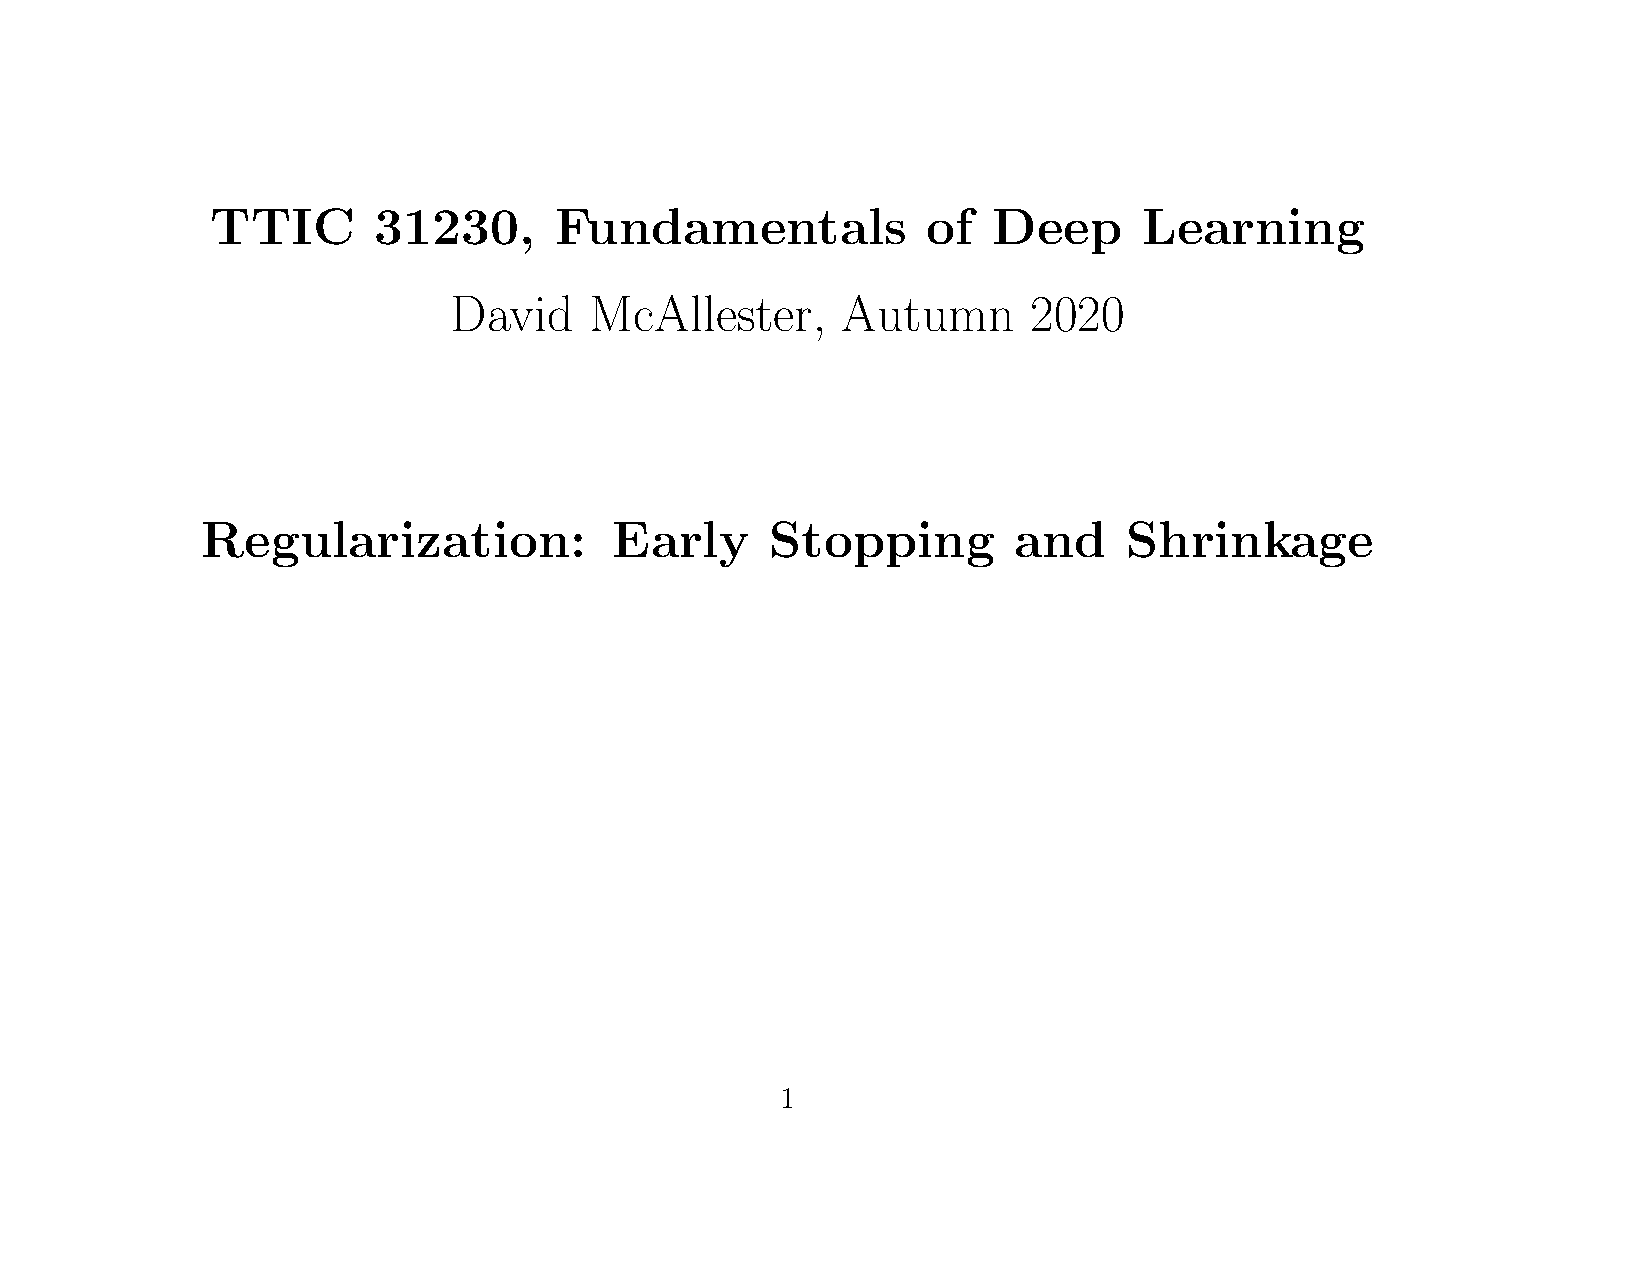
\includegraphics[height = 2in]{\images/Early}}

\vfill
Validation error is larger than training error when we stop.

\vfill
The model probabilities are tuned on training data statistics.

\vfill
The probabilities are tuned to an unrealistically low error rate and are therefore over-confident.

\vfill
This over-confidence occurs before the stopping point and damages validation loss (as opposed to validation error).

\slide{Shrinkage: $L_2$ regularization}

We first give a Bayesian derivation. We put a prior probability on $\Phi$ and maximize the a-posteriori probability (MAP).

\vfill
{\huge
\begin{eqnarray*}
\Phi^* & = & \argmax_\Phi\;p(\Phi | \tuple{x_1,y_1},\ldots,\tuple{x_n,y_n}) \\
\\
 & = & \argmax_\Phi\;\frac{p(\Phi,\; \tuple{x_1,y_1},\ldots,\tuple{x_n,y_n})}{p(\tuple{x_1,y_1},\ldots,\tuple{x_n,y_n})} \\
\\
 & = & \argmax_\Phi\;p(\Phi,\;\tuple{x_1,y_1},\ldots,\tuple{x_n,y_n})
 \end{eqnarray*}
}

\slideplain{5. Ensembles}

Train several models $\mathrm{Ens} = (\Phi_1,\;\ldots,\; \Phi_K)$ from different initializations and/or under different meta parameters.

\vfill
We define the ensemble model by

$$P_\mathrm{Ens}(y|x) = \frac{1}{K} \sum_k\; P_{\Phi_k}(y|x) = E_k \;P_k(y|x)$$

\vfill
Ensemble models almost always perform better than any single model.

\vfill
\slide{Ensembles Under Cross Entropy Loss}

\begin{eqnarray*}
{\cal L}\left(P_\mathrm{Ens}\right) & = & E_{\tuple{x,y} \sim \pop}\;\;-\ln P_\mathrm{Ens}(y|x) \\
\\
 & = & E_{\tuple{x,y} \sim \pop}\left[-\ln E_k\left[ P_k(y|x)\right]\right] \\
\\
& \leq & E_{\tuple{x,y} \sim \pop} \;E_k\left[-\ln P_k(y|x)\right] \\
\\
& = & E_k\; {\cal L}(P_k)
\end{eqnarray*}

\slide{Ensembles Under Cross Entropy Loss}

It is important to note that

$$-\ln E_k \;P_k(y|x) \;\;\leq E_k \left[-\ln P_k(y|x)\right]$$

\vfill
for each individual pair $\tuple{x,y}$.

\vfill
$\forall z\; f(z) \leq g(z)$ is stronger than $(E_z\;f(z)) \leq (E_z\; g(z))$.

\vfill
This may explain why in practice an ensemble model is typically better than any single component model.

\slide{6. Double Descent}

{\huge
Reconciling modern machine learning practice and the bias-variance trade-off

\bigskip
Mikhail Belkin, Daniel Hsu, Siyuan Ma, Soumik Mandal, arXiv December 2018.

\vfill
Deep Double Descent: Where Bigger Models and More Data Hurt

\bigskip
Preetum Nakkiran, Gal Kaplun, Yamini Bansal, Tristan Yang, Boaz Barak, Ilya Sutskever, ICLR 2020
}

\slide{Double Descent}

\centerline{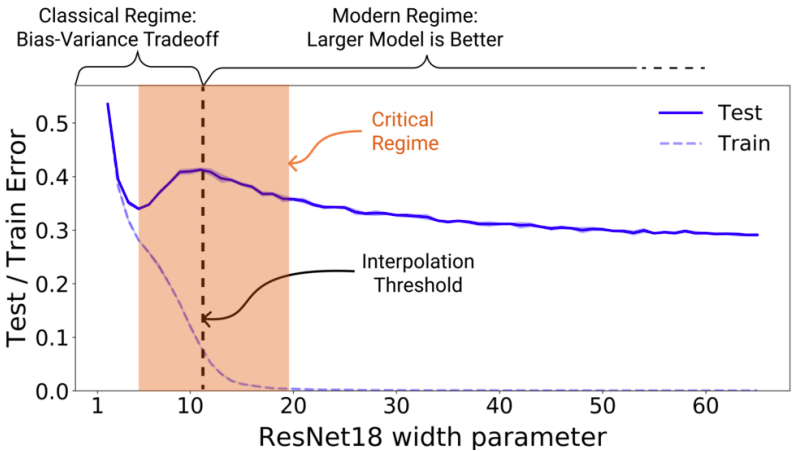
\includegraphics[width = 6in]{\images/DoubleDescent1}}

\vfill
Deep Double Descent: Where Bigger Models and More Data Hurt

\bigskip
Preetum Nakkiran, Gal Kaplun, Yamini Bansal, Tristan Yang, Boaz Barak, Ilya Sutskever, ICLR 2020

\slide{Double Descent}

\centerline{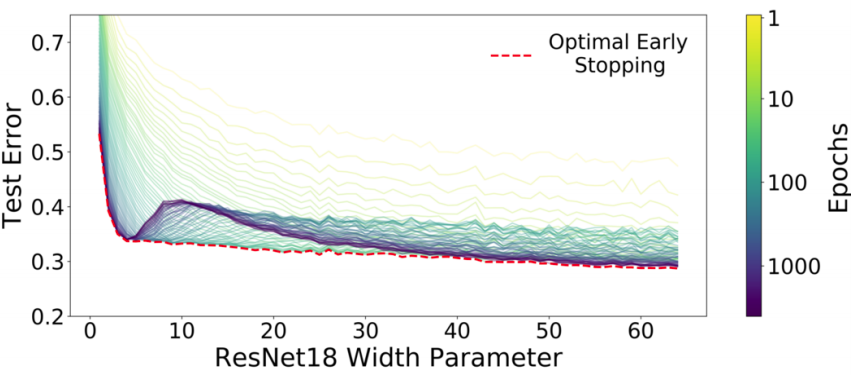
\includegraphics[width = 8in]{\images/DoubleDescent2}}

\slide{7. Grokking}

Power et al. {bf Grokking: Generalization Beyond Overfitting on Small Algorithmic Datasets [ArXiv 2201.02177]

\vfill
Wang et al. ``Grokked Transformers are Implicit Reasoners:
A Mechanistic Journey to the Edge of Generalization'' [arXiv 2405.15071]

\vfill
There is growing evidence that regularization ($L_2$ shrikage) over long runs lead to a ``phase transition''
reducing generalization loss late in training without improving the training loss.

\slide{END}

}
\end{document}
